% !TeX document-id = {f19fb972-db1f-447e-9d78-531139c30778}
% !BIB program = biber
\documentclass[compress]{beamer}
\usepackage[T1]{fontenc}
\usepackage{pifont}
\usetheme[block=fill,subsectionpage=progressbar,sectionpage=progressbar]{metropolis} 

\usepackage{wasysym}
\usepackage{etoolbox}
\usepackage[utf8]{inputenc}

\usepackage{threeparttable}
\usepackage{subcaption}

\usepackage{tikz-qtree}
\setbeamercovered{still covered={\opaqueness<1->{5}},again covered={\opaqueness<1->{100}}}


\usepackage{listings}

\lstset{
	basicstyle=\scriptsize\ttfamily,
	columns=flexible,
	breaklines=true,
	numbers=left,
	%stepsize=1,
	numberstyle=\tiny,
	backgroundcolor=\color[rgb]{0.85,0.90,1}
}



\lstnewenvironment{lstlistingoutput}{\lstset{basicstyle=\footnotesize\ttfamily,
		columns=flexible,
		breaklines=true,
		numbers=left,
		%stepsize=1,
		numberstyle=\tiny,
		backgroundcolor=\color[rgb]{.7,.7,.7}}}{}


\lstnewenvironment{lstlistingoutputtiny}{\lstset{basicstyle=\tiny\ttfamily,
		columns=flexible,
		breaklines=true,
		numbers=left,
		%stepsize=1,
		numberstyle=\tiny,
		backgroundcolor=\color[rgb]{.7,.7,.7}}}{}



\usepackage[american]{babel}
\usepackage{csquotes}
\usepackage[style=apa, backend = biber]{biblatex}
\DeclareLanguageMapping{american}{american-UoN}
\addbibresource{../../literature.bib }
\renewcommand*{\bibfont}{\tiny}

\usepackage{tikz}
\usetikzlibrary{shapes,arrows,matrix}
\usepackage{multicol}

\usepackage{subcaption}

\usepackage{booktabs}
\usepackage{graphicx}

\graphicspath{{../../pictures/}}

\makeatletter
\setbeamertemplate{headline}{%
	\begin{beamercolorbox}[colsep=1.5pt]{upper separation line head}
	\end{beamercolorbox}
	\begin{beamercolorbox}{section in head/foot}
		\vskip2pt\insertnavigation{\paperwidth}\vskip2pt
	\end{beamercolorbox}%
	\begin{beamercolorbox}[colsep=1.5pt]{lower separation line head}
	\end{beamercolorbox}
}
\makeatother



\setbeamercolor{section in head/foot}{fg=normal text.bg, bg=structure.fg}



\newcommand{\question}[1]{
	\begin{frame}[plain]
		\begin{columns}
			\column{.3\textwidth}
			\makebox[\columnwidth]{
				
\includegraphics[width=\columnwidth,height=\paperheight,keepaspectratio]{mannetje.png}}
			\column{.7\textwidth}
			\large
			\textcolor{orange}{\textbf{\emph{#1}}}
		\end{columns}
\end{frame}}

\newcommand{\instruction}[1]{\emph{\textcolor{gray}{[#1]}}}



\title[ML in PYthon]{\textbf{A Practical Introduction to Machine Learning in Python} \\Day 5 -- Friday \\ »Transformers«}
\author[Damian Trilling, Anne Kroon]{Damian Trilling \\ Anne Kroon \\ ~ \\ \footnotesize{d.c.trilling@uva.nl, @damian0604 \\a.c.kroon@uva.nl, @annekroon} \\}
\date{September 29, 2023}
\institute[Gesis]{Gesis}



\begin{document}

\begin{frame}{}
	\titlepage
\end{frame}

\begin{frame}{This part: State of the art and next steps}
	\tableofcontents
\end{frame}

\setbeamercovered{transparent}

\section{One-Hot to Continous}

\begin{frame}{Our BOW approach until now}
	\begin{block}{Representing a document by word frequency counts}
		Result of preprocessing and vectorizing:
		
		0. \texttt{He took the dog for a walk to the dog playground}\\
		$\Rightarrow$ \texttt{took dog walk dog playground}\\
		$\Rightarrow$ \texttt{'took':1, 'dog': 2, walk: 1, playground: 1}
	\end{block}
	
	Consider these other sentences
	\begin{enumerate}
		\item<2-> He took the doberman for a walk to the dog playground
		\item<3-> He took the cat for a walk to the dog playground
		\item<4-> He killed the dog on his walk to the dog playground 
	\end{enumerate}
	
	\onslide<5>{The vectorized representations of these sentences have a ``distance'' (dissimilarity) of 1 each, but arguably, sentences 0 and 1 should be ``closer'' than others}
\end{frame}

\subsection{Encoding text in ML models}

\begin{frame}{Encoding so far: BoW approach}
	\begin{itemize}
		\item Our vectorizers gave a random ID to each word
		\item Words are \emph{discrete} and \emph{independent} tokens.
		\item This is a rather naïve assumption, with two main disadvantages:
\begin{enumerate}
	\item high dimensionality of the \emph{one-hot-encodings} of the tokens
	\item they do not incorporate real-world knowledge
\end{enumerate}
	\end{itemize}

\begin{center}
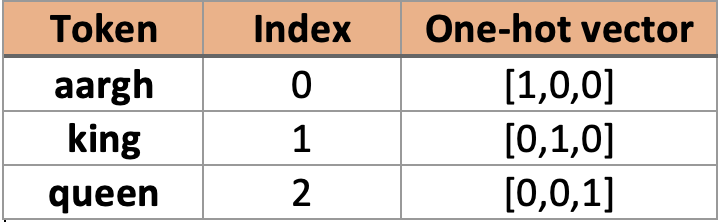
\includegraphics[scale=0.5]{bow.png}
\end{center}
\end{frame}

\begin{frame}{Continous vectors}
	\begin{itemize}
		\item A more realistic view: words are continous vectors in an N dimensional space
		\item Their representation contains real numbers, and they can occupy a position in the N dimensionality space
		\item This way of \emph{embedding} tokens is refered to as \emph{continous} or \emph{distributed} vectors, representations or \emph{word embeddings}
		\item The dimensions encode meaning (implicit)
		\end{itemize}
\end{frame}

\begin{frame}
\begin{center}
	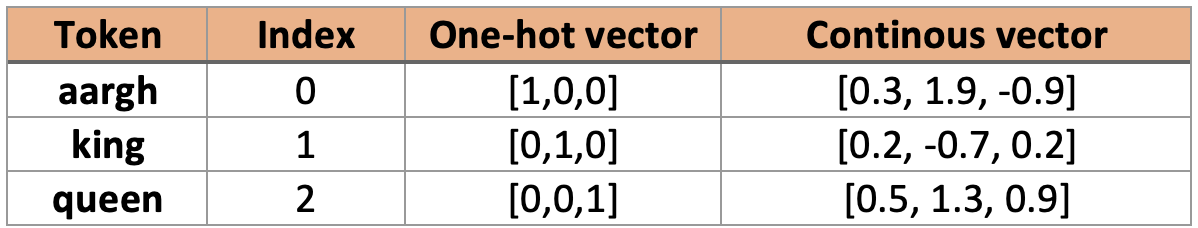
\includegraphics[scale=0.5]{bow_continous.png}
\end{center}
\end{frame}

\section{Language Modeling}

\begin{frame}
Language modelling refers to a set of techniques that aim determine the probability of a given sequence of words occurring in a sentence.
\end{frame}

\begin{frame}{Large Language Models}
	\begin{itemize}
		\item Often referred to as `pretrained' or `foundation' models.
		\item They rely on massive amounts of training data. 
		\item e.g., wikipedia, news archives, Reddit, etc. 
	\end{itemize}
\end{frame}

\begin{frame} {Training language models: based on unstructured text -- in the absence of explicit labels}
	\begin{figure}
		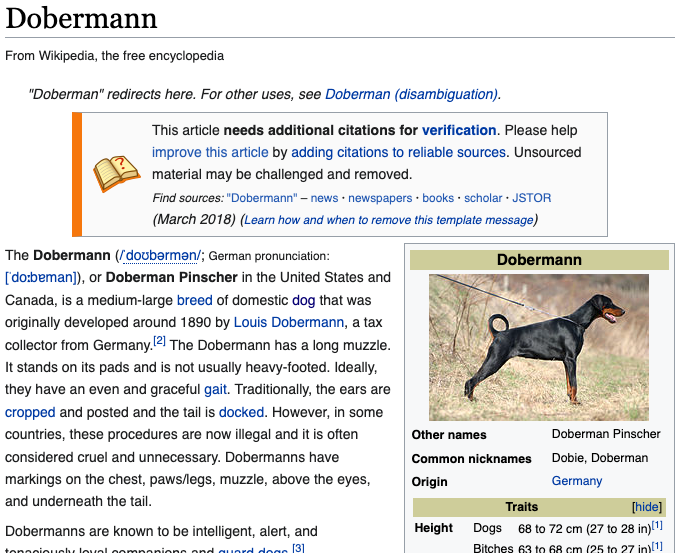
\includegraphics[width=0.475\textwidth]{dobermann.png}
		\hfill
		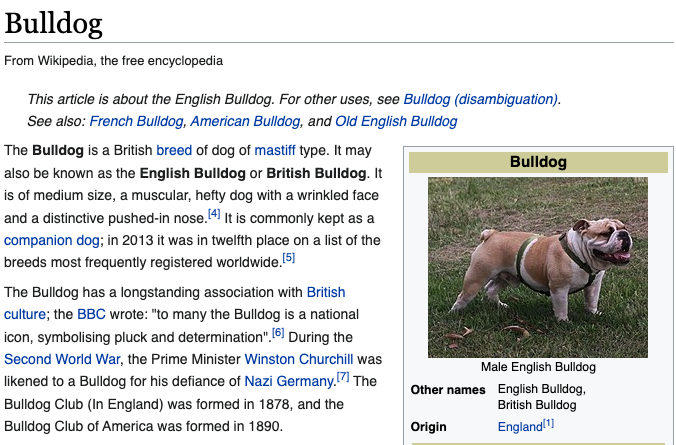
\includegraphics[width=0.475\textwidth]{bulldog.png}
	\end{figure}
\end{frame}

\begin{frame}{Key events in the history of language modeling}
		\makebox[\linewidth]{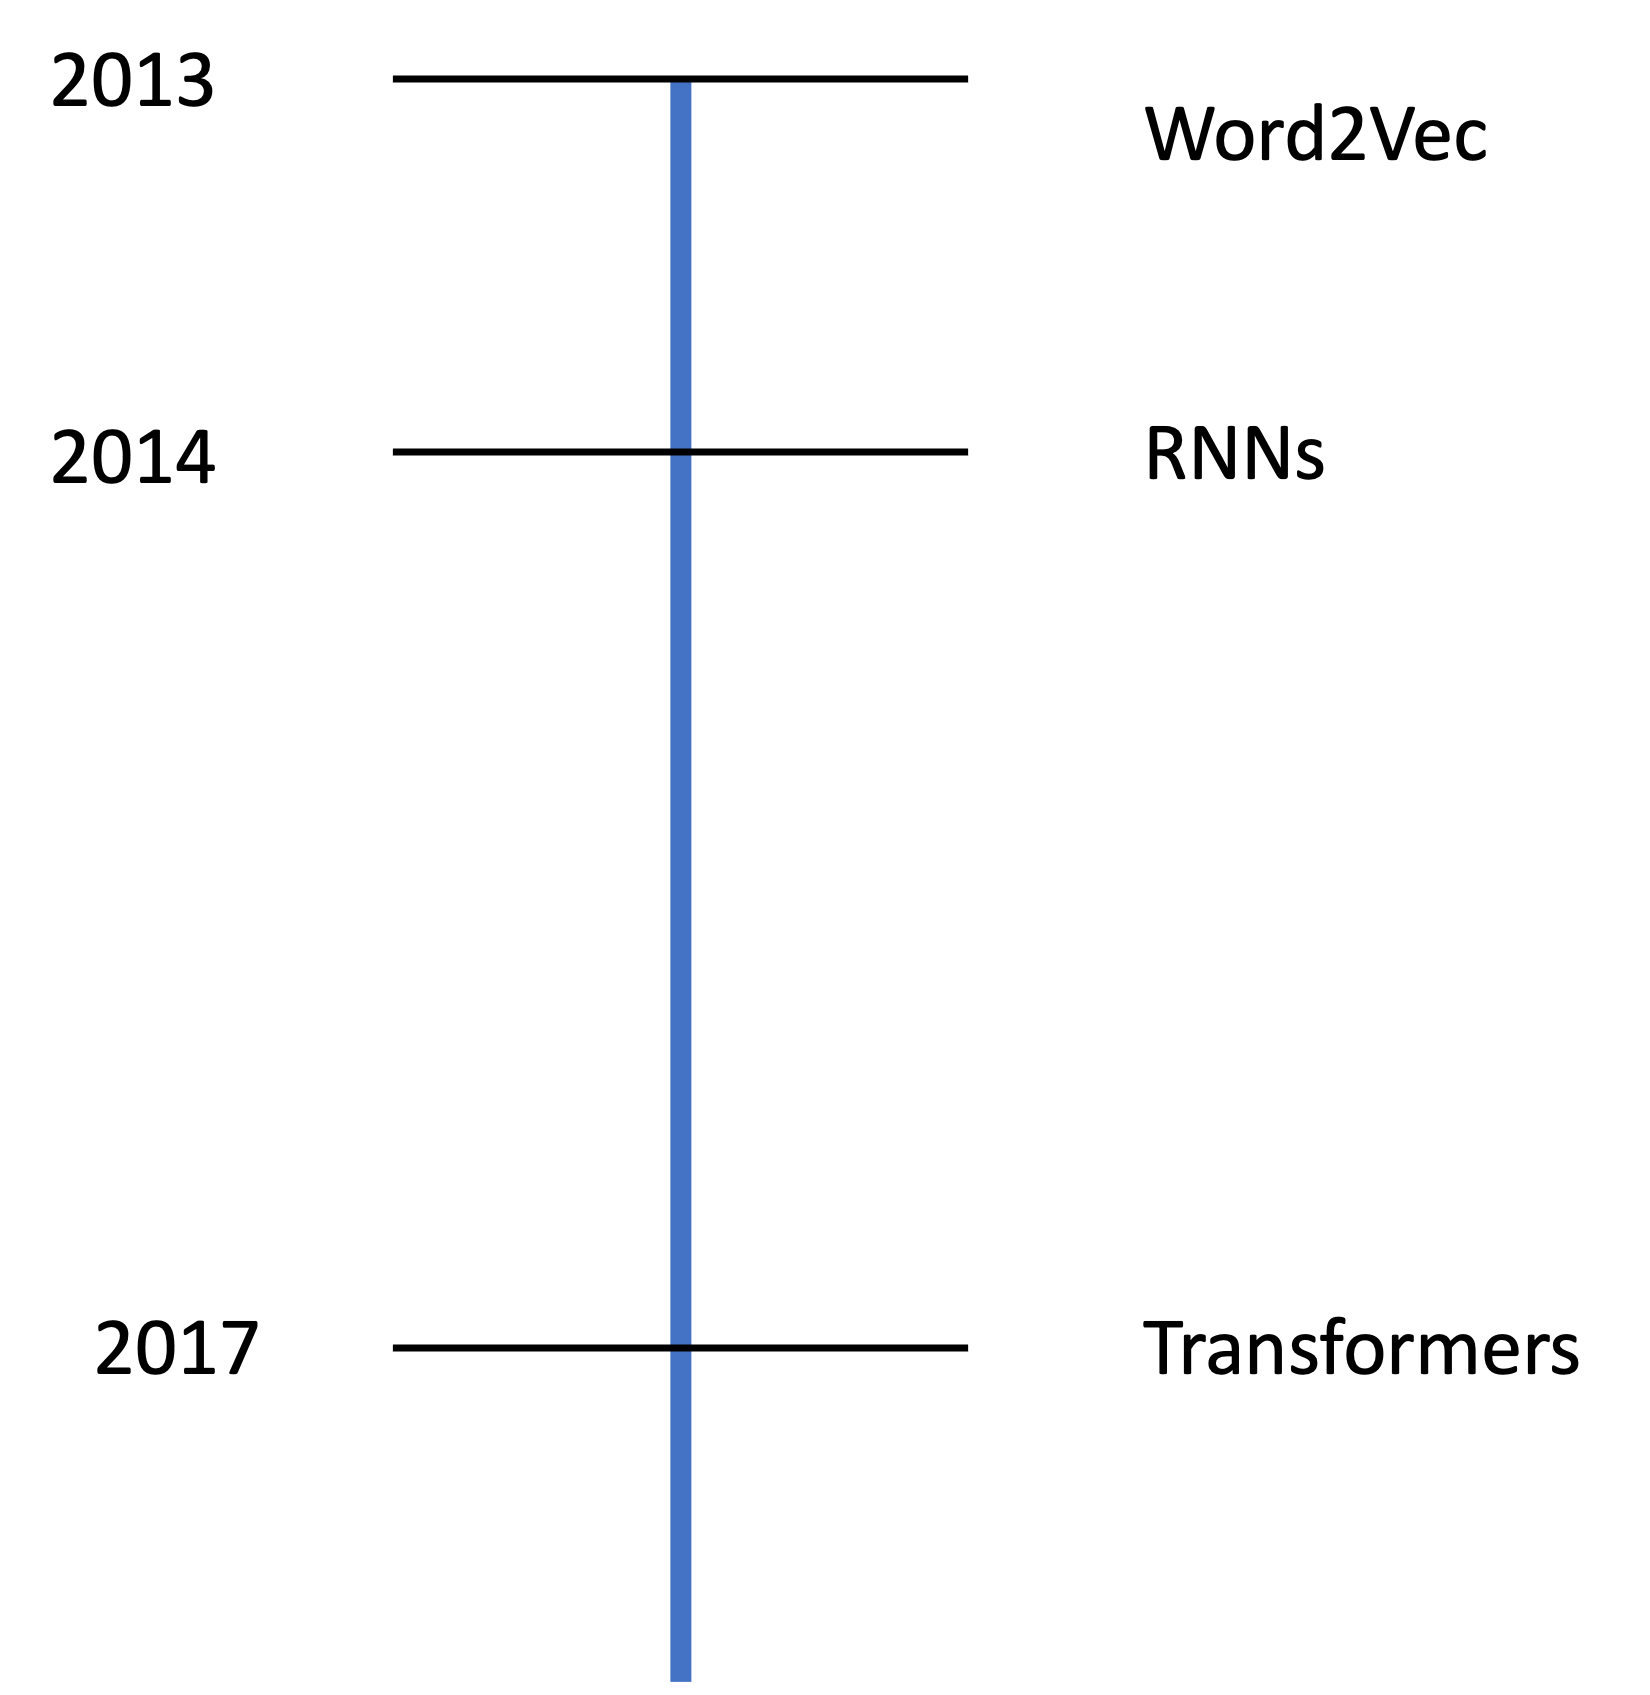
\includegraphics[width=\linewidth,height=\textheight, keepaspectratio]{language-modelling.png}}
\end{frame}


\section{Non-Contextual \\Embeddings}

\begin{frame}{``...a word is characterized by the company it keeps...'' (Firth, 1957)}
	\begin{block}{Word embeddings \ldots}
		\begin{itemize}
			\item help capturing the meaning of text
			\item are low-dimensional vector representations that capture semantic meaning
			\item for instance, `dobermann' and `bulldog' should be represented by vectors that are close to each other in space, while `kill' and `walk' should be far from each other.
		\end{itemize}
	\end{block}
\end{frame}


\begin{frame}{Word embeddings:Training algorithms}
	There are two popular approaches to training word embeddings: GloVe and word2vec.
	\begin{itemize}
		\item GloVe is count-based: dimensionality reduction on the co-occurrence counts matrix.
		\item Word2Vec is a predictive model: neural network to predict words/contexts
		\item That means that GloVe takes global context into account, word2vec local context
		\item Some technical implications for how training can be implemented 
		\item \textbf{However, only subtle differences in final result.}
	\end{itemize}
	
\end{frame}

\begin{frame}{Word2Vec: Continous Bag of Words (CBOW) vs skipgram}
	Example sentence: ``the quick brown fox jumped over the lazy dog''
	\begin{block}{CBOW: Predict a word given its context}
		Dataset:
		
		\texttt{([the, brown], quick), ([quick, fox], brown), ([brown, jumped], fox), ...}
	\end{block}
	
	\pause
	
	
	\begin{block}{skipgram: Predict the context given the word}	
		\texttt{(quick, the), (quick, brown), (brown, quick), (brown, fox), ...}
	\end{block}
	
	\tiny{Example taken from here: \url{https://medium.com/explore-artificial-intelligence/word2vec-a-baby-step-in-deep-learning-but-a-giant-leap-towards-natural-language-processing-40fe4e8602ba}}
\end{frame}

%window sizes


\begin{frame}{Continous Bag of Words (CBOW) vs skipgram}
	\begin{itemize}
		\item CBOW is faster
		\item skipgram works better for infrequent words
		\item Both are often used
		\item Usually, we use larger window sizes (e.g, 5)
		\item We need to specify the number of dimensions (typically 100--300)
	\end{itemize}
	\pause
	
	\textit{In any event, as a result of the prediction task, we end up with a \{100|200|300\}-dimensional vector representation of each word.*}
	
	
	\tiny{* If that makes you think of PCA/SVD, that's not completely crazy, see Levy, O., Goldberg, Y., \& Dagan, I. (2018). Improving Distributional Similarity with Lessons Learned from Word Embeddings. \textit{Transactions of the Association for Computational Linguistics, 3}, 211--225. doi:10.1162/tacl\_a\_00134}\\
\end{frame}


%Due to developments in the field of NLP, algorithms have become increasingly apt to understand human language. Word embeddings are the current state of the art for capturing the meaning of texts. Word embeddings are vector representations of words. They are the current state of the art in NLP to understand, capture and process language. The basic idea of word embeddings is that one gets to know a word by looking at the company that it keeps; contexts is crucial in understanding word meaning. 


\begin{frame}{You can literally calculate with words!}
	And answer questions such as ``Man is to woman as king is to \_\_\_\_?''
	\makebox[\linewidth]{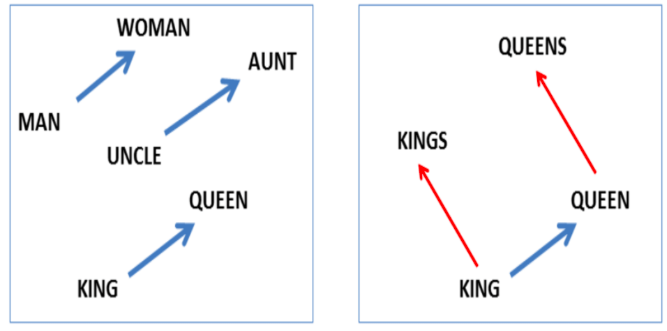
\includegraphics[width=\linewidth,height=\textheight, keepaspectratio]{embeddings.png}}
	semantic relationships vs. syntactic relationships
\end{frame}

%word vectors that are able to capture the relationships between words in a surprisingly expressive way. Word embeddings are especially effective in understanding analogies, and for example understand that man is to woman as uncle to aunt, and king to king. 

\subsection[Improving down-stream classification tasks]{Using word embeddings to improve models}
\begin{frame}[plain]
	Using word embeddings to improve down-stream classification tasks.
\end{frame}

\begin{frame}{In supervised machine learning}
	\begin{itemize}[<+->]
		\item Modify CountVectorizer or TfIdfVector such that for each term, you do not only count how often it occurs, but also multiply with its embedding vector
		\item Often, pre-trained embeddings (e.g., trained on the whole wikipedia) are used
		\item Thus, our supervised model will be able to deal with synonyms and related words!
	\end{itemize}
	

	
\end{frame}



\begin{frame}[plain]
	\makebox[\linewidth]{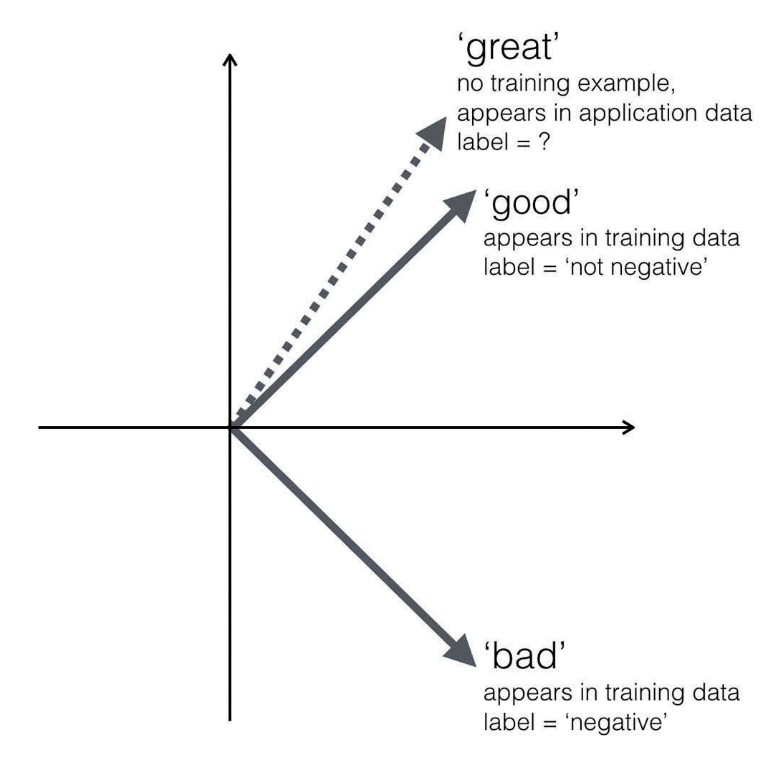
\includegraphics[width=\linewidth,height=\textheight, keepaspectratio]{rudkowsky2018-1}}
	
	\tiny{Rudkowsky, E., Haselmayer, M., Wastian, M., Jenny, M., Emrich, Š., \& Sedlmair, M. (2018). More than Bags of Words: Sentiment Analysis with Word Embeddings. \textit{Communication Methods and Measures, 12}(2–3), 140–157. doi:10.1080/19312458.2018.1455817}
\end{frame}


\begin{frame}{It's not always black/white\ldots}
	Sometimes, BOW may be just fine (for very negative sentences, it doesn't matter). But especially in less clear cases ('slightly negative'), embeddings increased performance.
	\makebox[\linewidth]{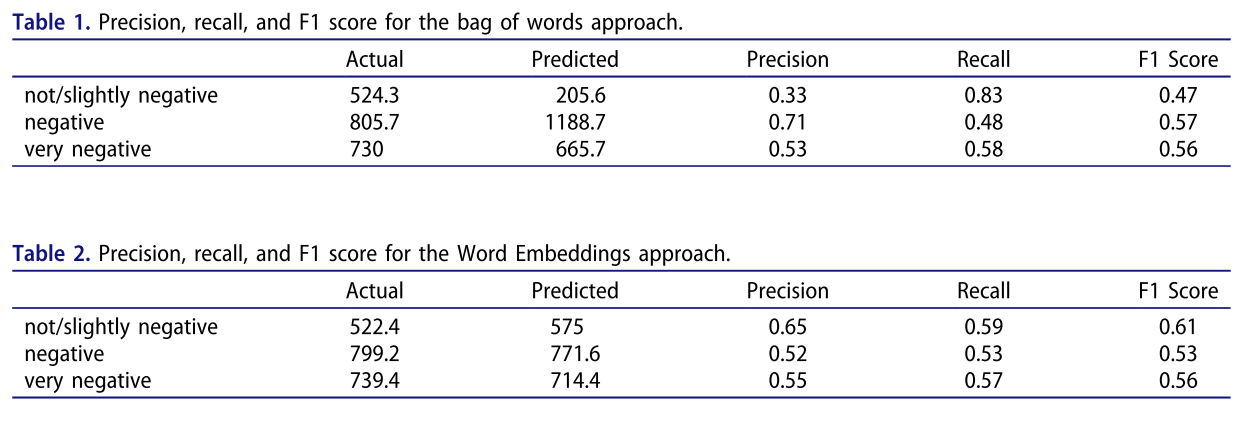
\includegraphics[width=\linewidth,height=\textheight, keepaspectratio]{rudkowsky2018-2}}
	
	\vfill
	
	\tiny{Rudkowsky, E., Haselmayer, M., Wastian, M., Jenny, M., Emrich, Š., \& Sedlmair, M. (2018). More than Bags of Words: Sentiment Analysis with Word Embeddings. \textit{Communication Methods and Measures, 12}(2–3), 140–157. doi:10.1080/19312458.2018.1455817}
\end{frame}


\begin{frame}{In document similarity calculation}
	\begin{block}{Use cases}
		\begin{itemize}
			\item plagiarism detection
			\item Are press releases/news agency copy/\ldots taken over?
			\item Event detection
		\end{itemize}
	\end{block}
	\pause
	\begin{block}{Traditional measures}
		\begin{itemize}
			\item Levenshtein distance (How many characters|words do I need to change to transform string A into string B?)
			\item Cosine similarity (``correlation'' between the BOW-representations of string A and string B)
		\end{itemize}
	\end{block}
\end{frame}


\begin{frame}[plain]
	BUT: This only works for literal overlap. What if the writer chooses synonyms?
	\pause 
	
	\makebox[\linewidth]{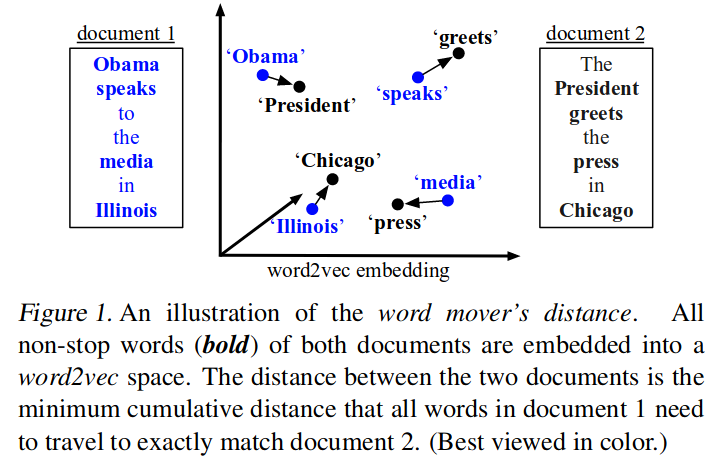
\includegraphics[width=\linewidth,height=\textheight, keepaspectratio]{wmd}}
	
	
	\tiny{Kusner, M. J., Sun, Y., Kolkin, N. I., \& Weinberger, K. Q. (2015). From Word Embeddings To Document Distances. \textit{Proceedings of The 32nd International Conference on Machine Learning} (Vol. 37, pp. 957–966)}
\end{frame}


\begin{frame}{There are several approaches}
	\begin{itemize}
		\item word mover's distance
		\item soft cosine similarity
	\end{itemize}
	In common: we use pre-trained embeddings to replace words (that otherwise would just have a random identifier and be unrelated) with vectors representing their meaning, when calculating our measure of interest
\end{frame}

\section{Neural networks}


\begin{frame}{Neural Networks}
	\begin{itemize}
		\item In ``classical'' machine learning, we predict an outcome directly based on the input features
		\item In neural networks, we can have ``hidden layers'' that we predict
		\item These layers are not necessarily interpretable
		\item ``Neurons'' that ``fire'' based on an ``activation function''
	\end{itemize}
	
\end{frame}

\begin{frame}
	
	\def\layersep{2.5cm}
	
	\begin{tikzpicture}[shorten >=1pt,->,draw=black!50, node distance=\layersep]
		\tikzstyle{every pin edge}=[<-,shorten <=1pt]
		\tikzstyle{neuron}=[circle,fill=black!25,minimum size=17pt,inner sep=0pt]
		\tikzstyle{input neuron}=[neuron, fill=green!50];
		\tikzstyle{output neuron}=[neuron, fill=red!50];
		\tikzstyle{hidden neuron}=[neuron, fill=blue!50];
		\tikzstyle{annot} = [text width=4em, text centered]
		
		% Draw the input layer nodes
		\foreach \name / \y in {1,...,4}
		% This is the same as writing \foreach \name / \y in {1/1,2/2,3/3,4/4}
		\node[input neuron, pin=left:Input \#\y] (I-\name) at (0,-\y) {};
		
		% Draw the hidden layer nodes
		\foreach \name / \y in {1,...,5}
		\path[yshift=0.5cm]
		node[hidden neuron] (H-\name) at (\layersep,-\y cm) {};
		
		
		% Draw the output layer node
		\node[output neuron,pin={[pin edge={->}]right:Output}, right of=H-3] (O) {};
		
		% Connect every node in the input layer with every node in the
		% hidden layer.
		\foreach \source in {1,...,4}
		\foreach \dest in {1,...,5}
		\path (I-\source) edge (H-\dest);
		
		% Connect every node in the hidden layer with the output layer
		\foreach \source in {1,...,5}
		\path (H-\source) edge (O);
		
		% Annotate the layers
		\node[annot,above of=H-1, node distance=1cm] (hl) {Hidden layer};
		\node[annot,left of=hl] {Input layer};
		\node[annot,right of=hl] {Output layer};
	\end{tikzpicture}
	
	$\Rightarrow$ If we had multiple hidden layers in a row, we'd call it a \emph{deep} network.
\end{frame}


\begin{frame}{Why neural networks?}
	\begin{itemize}
		\item learn hidden structures (e.g., embeddings (!))
		\item go beyond the idea that there is a direct relationship between occurrence of word X and label (or occurrence of pixel [R,G,B] and a label)
		\item images, machine translation --- and more and more general NLP, sentiment analysis, etc.
	\end{itemize}
	
	\small {Example of a comparatively easy introduction:
		\url{https://towardsdatascience.com/neural-network-embeddings-explained-4d028e6f0526}}
	
\end{frame}


\begin{frame}[fragile]{Simple feed forward network}
	\begin{lstlisting}
model.add(Dense(300, input_dim=input_dim, activation='relu'))
model.add(Dense(1, activation='sigmoid'))
	\end{lstlisting}	
	
	\begin{itemize}[<+->]
		\item Our first layer reduces the input features (e.g., the 10,000 features our CountVectorizer creates) to 300 neurons
		\item It does so using the relu function $f(x) = max(0, x)$ (as our counts cannot be negartive, just a linear function)
		\item The second layer reduces the 300 neurons to 1 output neuron using the sigmoid function (the S curve you know fron logistic regression)
		\item Of course, we can add multiple layers in between if we want to
	\end{itemize}
\end{frame}



\begin{frame}{Convolutional networks}
	The problem with such a basic networks: just as with classic SML, we still loose all information about order (the ``not good'' problem).
	
	Therefore,
	\begin{itemize}
		\item We concatenate the vectors of neighboring words
		\item We apply some filter (essentially, we detect patterns)
		\item and then pool the results (e.g., taking the maximum)
	\end{itemize}
	This means that we now excplitly take into acount \emph{the temporal structure} of a sentence.
\end{frame}



\begin{frame}{Convolutional networks}
	
	\makebox[\columnwidth]{
		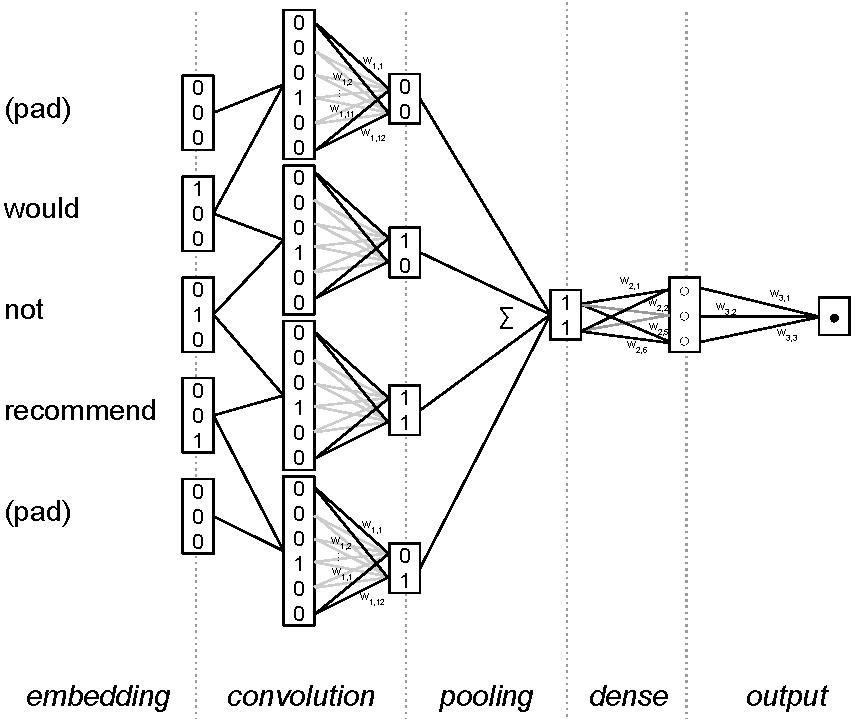
\includegraphics[width=\columnwidth,height=.8\paperheight,keepaspectratio]{ch09_cnn_cropped}}
\end{frame}



\begin{frame}[fragile]{Convolutional networks}
	\begin{lstlisting}
model.add(Embedding(input_dim=vocab_size, output_dim=embedding_dim, input_length=maxlen))
model.add(Conv1D(embedding_dim, 5, activation='relu'))
model.add(GlobalMaxPooling1D())
model.add(Dense(300, activation='relu'))
model.add(Dense(1, activation='sigmoid'))
		
	\end{lstlisting}	
	The layers:	
	\begin{enumerate}[<+->]
		\item train an embedding model
		\item apply the convolution with 5 ``timestamps''
		\item pool using the maximum
		\item another layer with 300 dimensions
		\item the final layer with 1 output neuron
	\end{enumerate}
\end{frame}


\begin{frame}{Convolutional networks}
	\textbf{Note that the preprocessing differs!}
	
	\begin{itemize}
		\item We do not take a word vector per document as input any more, but \emph{a sequence of words}
		\item For concatenating, these sequences need to have equal length, which is why we \emph{pad} then
	\end{itemize}
	
\end{frame}

\begin{frame}{LSTM (long short-term memory)}
	\begin{itemize}
		\item Unlike ``feed forward'' neural networks, this is  a ``recurrent neural network'' (RNN) -- the training works in two directions
		\item Heavy in computation, very useful for predicting \emph{sequences}
		\item Won't cover today
	\end{itemize}
\end{frame}


\subsection{Using pretrained embeddings}

\begin{frame}{The embedding layer}
	\begin{itemize}
		\item Often, the first layer is creating word embeddings
		\item Good embeddings need a lot of training data
		\item Training good embeddings needs time
		\item Therefore, we can replace that layer with a pre-trained embedding layer (!)
		\item We can even use a hybrid approach and allow the pre-trained embedding layer to be re-trained!
	\end{itemize}
\end{frame}

\section{Contextual Embeddings}

\begin{frame}
\begin{alertblock}{Downsides of Non-Contextual Word Embeddings}
	\begin{itemize}
		\item Word2Vec and Glove produce \emph{static} vectors: each word is represented by a single vector.
		\begin{itemize}	
\item e.g., the vector for \emph{date} is always the same...
\item ...however, the \emph{meaning} of this word differs across domains: ``she put a \emph{date} in his lunchbox'' (1); ``they went on a \emph{date}'' (2); and ``what's the \emph{date} today?"
		\end{itemize}
	\end{itemize}
\end{alertblock}
\begin{exampleblock}{Enter: Contextual Word Embeddings}
	\begin{itemize}
		\item \emph{Transformers} create a new vector for each time a word is used in the dataset
		\item \emph{Contextualized} vectors.
		\item \textit{self-attention} mechanism is essential here: this is a manner to automatically decide which nearby words should influence a token's representation; the model  \textit{learns} which tokens \emph{to attend to} 
	\end{itemize}
\end{exampleblock}
\end{frame}

\section{Transfer learning paradigm}

\begin{frame}{The idea of transfer learning is very powerful}
	\begin{block}{Transfer Learning paradigm}
		\begin{enumerate}
			\item \alert{Pre-train} a model on data that is at hand (e.g., Wikipedia, Google News)
			\item \alert{Fine-tune} the model on your downstream task (bring in your small-scale annotated dataset)
		\end{enumerate}
	By adding `task-specific' heads you can produce specific outputs, e.g., classification, text generation, named entity recognition, etc. 
	\end{block}
\end{frame}
	

\section{Transformer-based models}

\begin{frame}
	The architecture of transformers is very efficient on modern hardware; transformers process words in parallel.
	As they are much faster, we can use much more data. 
\end{frame}

\begin{frame}{Transformer-based models}
	\begin{block}{BERT: Bidirectional Encoder Representations from Transformers \parencite{BERT}}
		\begin{itemize}[<+->]
			\item (Huge) pre-trained model (by, e.g., Google) 
			\item Trained on very large amount of text and can use words in context. 
			\item State of the art performance on the General Language Understanding Evaluation benchmark (GLUE). 
			\item BERT and other transformer-based models are used for a range of tasks;
			\begin{enumerate}
				\item Sentiment analysis
				\item sequence-to-sequence predictions (e.g., translation)
				\item similarity and paraphrasing tasks
				\item natural language inference tasks
		\end{enumerate}
	\end{itemize}
	\end{block}
\end{frame}

\begin{frame}{How to use}
	\begin{block}{HuggingFace}
		\begin{itemize}[<+->]
			\item The `HuggingFace`: Python library includes lots of datasets and transformer-based models 
			\item `HuggingFace`'s API works well with libraries such as `TensorFlow`, `Keras`, and `PyTorch`. 
		\end{itemize}
	\end{block}
\end{frame}

\begin{frame}{Finding the pre-trained model that suits your needs}
	\begin{block}{HuggingFace}
		\begin{itemize}[<+->]
			\item The `HuggingFace`: Python library includes lots of datasets and transformer-based models 
			\item `HuggingFace`'s API works well with libraries such as `TensorFlow`, `Keras`, and `PyTorch`. 
		\end{itemize}
	\end{block}
\end{frame}

\begin{frame}[standout]
	Let's look at an example (exercises/transformers-custom-dataset.ipynb)
\end{frame}

\subsection{Do I need all this fancy stuff?}

\begin{frame}{Things to consider}
	How important is\ldots
	\begin{itemize}[<+->]
		\item precision/recall? Am I satisfied with .88 when .90 is theoretically possible? .85? .80? .75?
		\item explainability?
		\item computational resources?
		\item generalizability and out-of-sample performance?
	\end{itemize}
\end{frame}

\begin{frame}{Do I need all this fancy stuff?}
	\begin{itemize}[<+->]
		\item Always estimate a simple baseline model first
		\item Invest in good hyperparameter-tuning (cross-validation, gridsearch) and don't forget to set aside unseen data for the \emph{final} evaluation.
		\item If you (a) need to get the highest possible accuracy, or (b) have reasons to assume that the model does not generalize well enough (overfitting problems, bad out-of-sample prediction (e.g., training topics on newspaper 1, predicting topics in newspaper 2), try embedding-based approaches, transformers, etc.
		\item Rule of thumb: the more abstract/latent what you want to predict, the less likely classic ML is going to work
	\end{itemize}
\end{frame}


\section{Ethical considerations}

\begin{frame}[plain]
	(Ab-)using word embeddings to detect biases
\end{frame}

\begin{frame}{Biased embeddings}
	\begin{itemize}
		\item word embeddings are trained on large corpora
		\item As the task is to learn how to predict a word from its context (CBOW) or vice versa (skip-gram), biased texts produce biased embeddings
		\item If in the training corpus, the words ``man'' and ``computer programmer'' are used in the same context, then we will learn such a gender bias
	\end{itemize}
	
	\tiny{Bolukbasi, T., Chang, K.-W., Zou, J., Saligrama, V., \& Kalai, A. (2016). Man is to Computer Programmer as Woman is to Homemaker? Debiasing Word Embeddings, 1–25. Retrieved from http://arxiv.org/abs/1607.06520}
\end{frame}


\begin{frame}{Biased embeddings}
	Usually, we do not want that (and it has a huge potential for a shitstorm)
	
	~\\
	\pause
	
	unless\ldots
	
	~\\
	\pause
	
	we actually want to chart such biases.
	
\end{frame}


\begin{frame}{An exmaple from our research}
We trained word embeddings on 3.3 million Dutch news articles.
	
Are vector representations of outgroups (Maroccans, Muslims) closer to representations of negative stereotype words than ingroups?
\vspace{.5cm}
	
\tiny{Kroon, A.C., Van der Meer, G.L.A., Jonkman, J.G.F., \&Trilling, D. (in press): Guilty by Association: Using Word Embeddings to Measure Ethnic Stereotypes in News Coverage. \emph{Journalism \& Mass
			Communication Quarterly}}
\end{frame}


\begin{frame}[plain]
	\makebox[\linewidth]{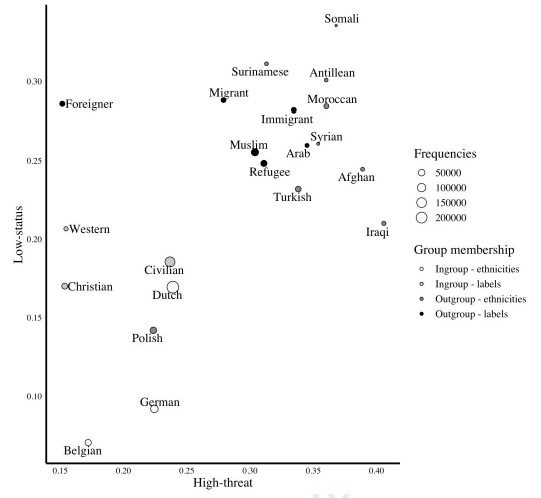
\includegraphics[width=\linewidth,height=\textheight, keepaspectratio]{embeddingbias}}
	
\end{frame}




\section{Your takeaway}


\begin{frame}[standout]
(short recap of course)
\end{frame}


\question{Have your plans about how to and wether to use ML changed? }


\question{What are your next steps?}


\begin{frame}[standout]
Last part: we help you working on (or discussing about) your own projects.
\end{frame}


\section[AEM]{AEM: An application from our own research}

\begin{frame}[plain]
	We can use pre-trained embeddings -- but can we make even better ones?
	\textbf{The Amsterdam Embedding Model (AEM)}\\
	
	
	\vspace{1cm}
	
	{\footnotesize{Anne Kroon, Antske Fokkens, Damian Trilling, Felicia Loecherbach, Judith Moeller, Mariken A. C. G. van der Velden, Wouter van Atteveldt} }
\end{frame}



%For all these tasks, you need to process text. 
%Humans are obviously very good in this. However, we are not capable of handling %humongous amounts of data. Therefore, we need computers. 
%For computers, it used to be relatively hard to understand language, to capture %semantic relations, especially in different type of contexts. 


\begin{frame}{Why do this?}
	\begin{itemize}
		\item Embedding models are of great interest to communication scholars
		\item yet... Most publicly available models represent \textbf{English} language
		\item The preparation of good-performing embedding models require a significant amount of \textbf{time} and \textbf{access to a large amount of data sets}
		\item Few Dutch embedding models are available, but trained on ordinary human language from the World Wide Web.
		\item These models do not capture the specifics of news article data and are therefore less suitable to study and understand dynamics of this domain
		\item $\Rightarrow$ No model is available trained on Dutch news data
	\end{itemize}
\end{frame}

%Properly trained embedding models are of great interest to communication scholars, because they can help with diverse tasks, such as topic classification, automated sentiment analysis or bias detection. Yet – currently no model exist that is trained on media data – and therefore effectively deals with the particularities of news media data. 

%\subsection{The Amsterdam Embedding Model}
\begin{frame}{Project's Aim}
	\begin{block}{Aim of the current project} 
		\begin{enumerate}
			\item Develop and evaluate a high-quality embedding model
			\item Assess performance in downstream tasks of interest to Communication Science (such as topic classification of newspaper data).
			\item Facilitate distribution and use of the model
			\item Offer clear methodological recommendations for researchers interested using our Dutch embedding model
		\end{enumerate}
	\end{block}
\end{frame}

%Therefore, this project was set out to develop a good word embedding model trained on Dutch media data, and facilitate its distribution


%\subsection{Approach and Preliminary Results}

\begin{frame}{Training data}
	\begin{block}{Training data set}
		\begin{itemize}
			\item Dataset: diverse print and online news sources
			\item Preprocessing: duplicate sentences were removed
			\item Telegraaf (print \& online), NRC Handelsblad (print \& online), Volkskrant (print \& online), Algemeen Dabldad (print \& online), Trouw (print \& online), nu.nl , nos.nl
			\item \# words: 1.18b (1181701742)
			\item \# sentences: 77.1M (77151321)
		\end{itemize}
	\end{block}
\end{frame}

\begin{frame}{Training model}
	\begin{block}{Training model}
		\begin{itemize}
			\item We trained the model using Gensim's Word2Vec package in Python
			\item Skip-gram with negative sampling, window size of 5, 300-dimensional word vectors
		\end{itemize}
	\end{block}
\end{frame}

%\subsection{Evaluation}
\begin{frame}{Evaluation}
	Evaluation of the Amsterdam Embedding Model
\end{frame}

\begin{frame}{Evaluation}
	\begin{block}{Evaluation methods}
		\begin{itemize}
			\item To evaluate the model, we compare it to two other publicly available embedding models
			\begin{itemize}
				\item $\Rightarrow$ \textbf {'Wiki'}: Embedding model trained on Wikipedia data (FastText)
				\item $\Rightarrow$ \textbf{'Cow'}: Embedding model trained on diverse .nl and .be sites (Schafer \& Bildhauer, 2012; Tulkens et al., 2016)
				\item $\Rightarrow$ \textbf{'AEM'}: Amsterdam Embedding Model
			\end{itemize}
		\end{itemize}
	\end{block}
\end{frame}

%To evaluate our model, we will compare it (at least in a first step) – to two other, publicly available word embedding models: One trained on Wikipedia data, and the other on divers dutch and Belgian websites. 

\begin{frame}{Evaluation data}
	\begin{block}{Evaluation data}
		\begin{enumerate}
			\item 'relationship'/ analogy-task (Tulkens et al., 2016)
			\begin{itemize}
				\item \textbf{syntatic relationships}: dans dansen loop \textit{[lopen]}
				\item \textbf{semantic relationships}: denemarken kopenhagen noorwegen \textit{[oslo]}
			\end{itemize}
			\item 5806 relationship tasks
		\end{enumerate}
	\end{block}
\end{frame}

%Tulkens et al created several Dutch relationship tasks. For example, when given dans (dance) dansen (dancing) and loop (walk), the computer has to guess that the word we are looking for is lopen (walking). This is an example of syntactic analogy. The same applies to capital - country relations (Copenhagen is to Denmark as … [Oslo] to Norway]. This is an example of a semantic analogy. 
%Each model had to solve over 5K of these types of analogy tasks. We subsequently use these results to compare how well they do.

\begin{frame}{}
	\makebox[\linewidth]{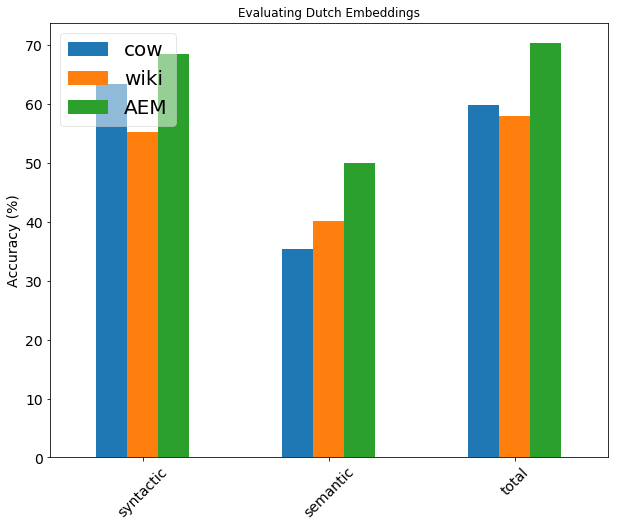
\includegraphics[width=\linewidth,height=\textheight, keepaspectratio]{evaluation_data.png}}
\end{frame}

%As can be seen, the AEM (= Amsterdam Embedding Model) outperfoms the other models on both syntactic analogies and semantic analogies. 

%\subsection{Illustration}
\begin{frame}{Illustration}
	Illustration - Using the Amsterdam Embedding Model
\end{frame}

%Let's see what the model has learned about Dutch language. Now, we will provide some illustrations of how well the AEM understands the Dutch language. More specifically, we will provide a 2 dimensional visualisation of some random Dutch words in the word vector space..


\subsection{}
\begin{frame}{}
	\makebox[\linewidth]{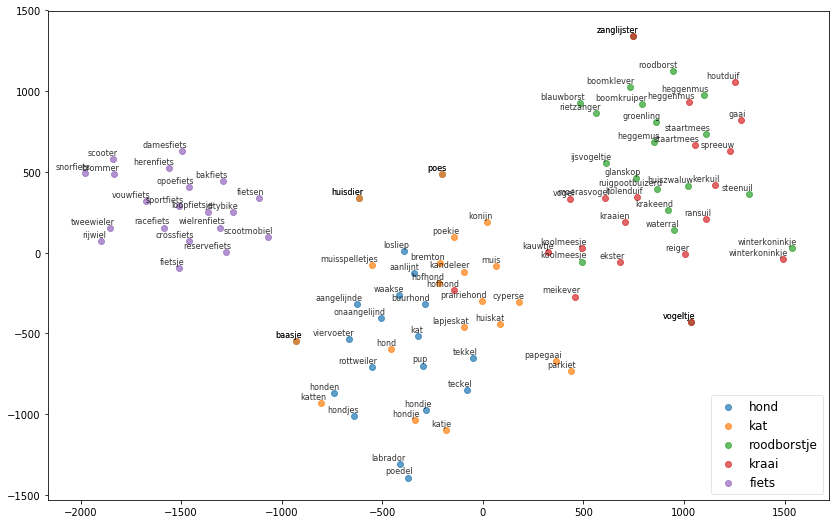
\includegraphics[width=\linewidth,height=\textheight, keepaspectratio]{w2v_300_illustration.png}}
\end{frame}

% this is a 2 dimensional representation of the most similar words to fiets, hond, kat, roodborstje and kraai 

\begin{frame}{}
	\makebox[\linewidth]{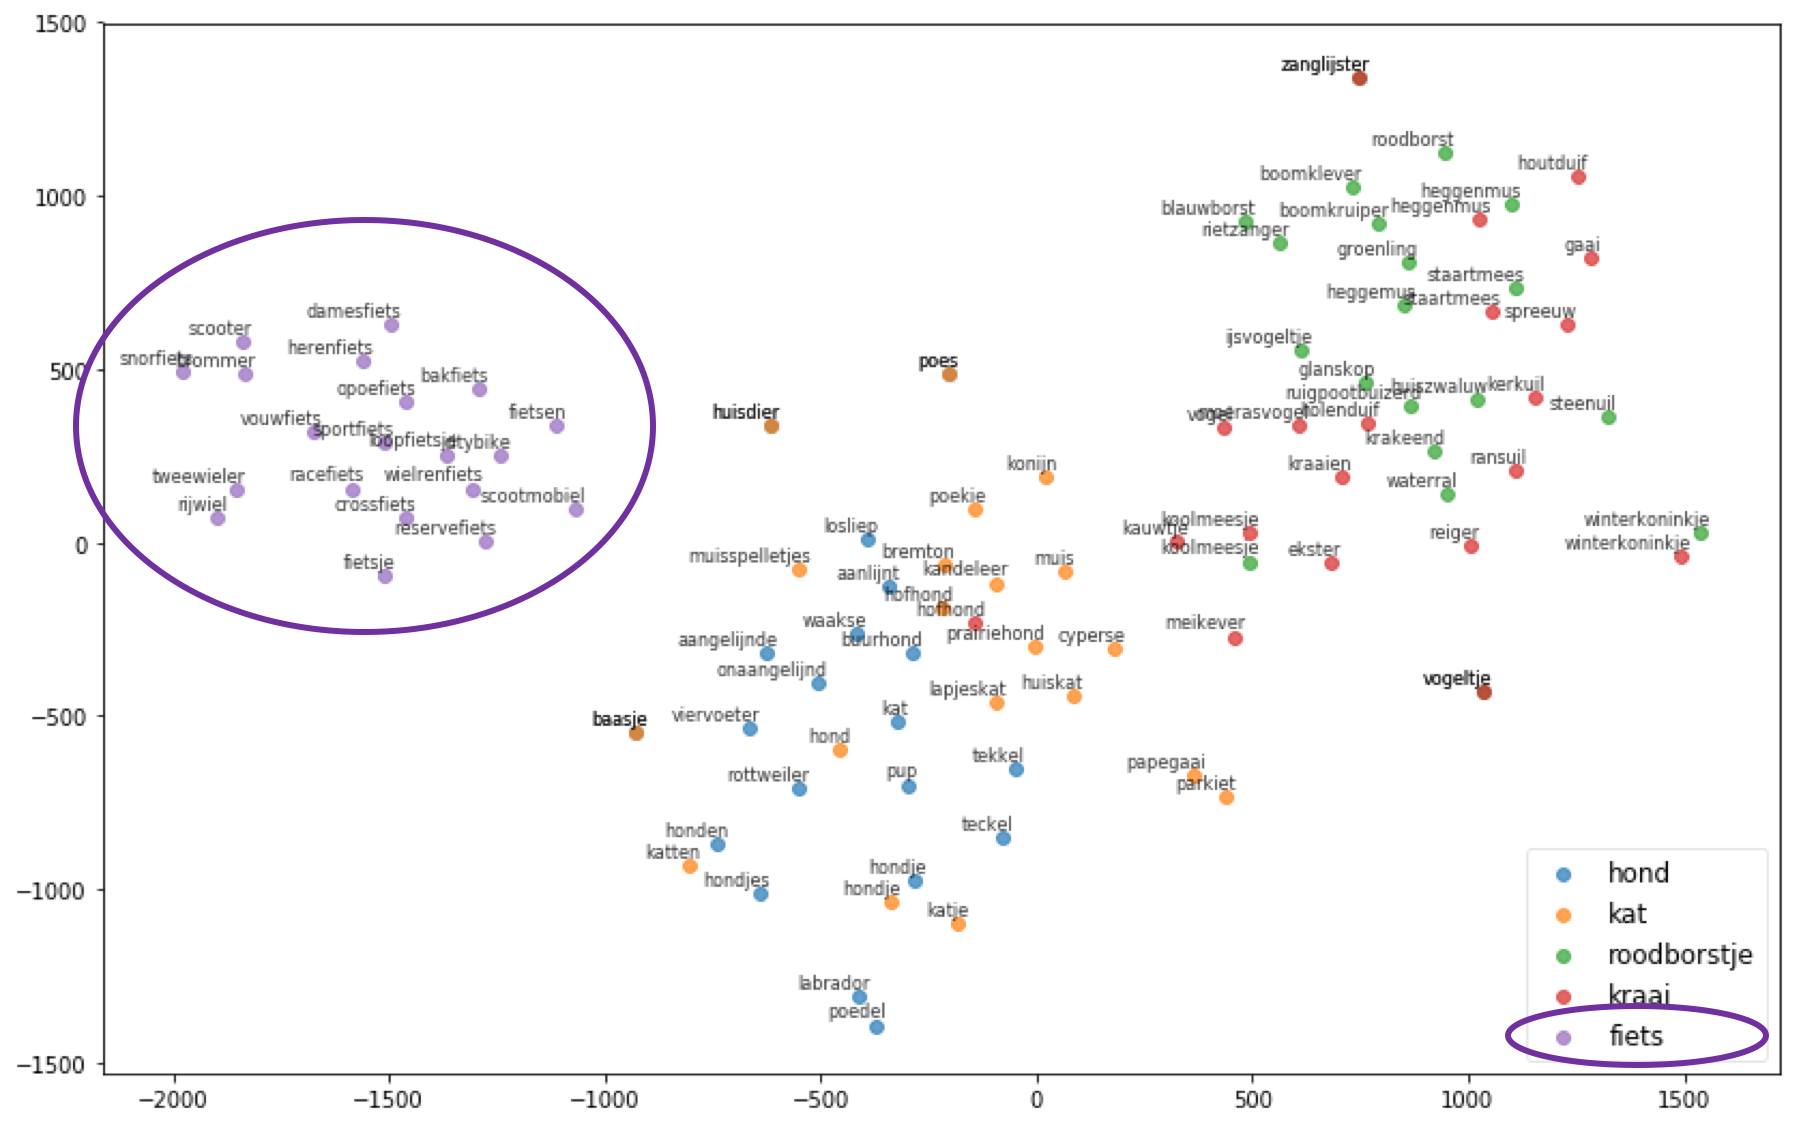
\includegraphics[width=\linewidth,height=\textheight, keepaspectratio]{visual2.png}}
\end{frame}

%as can be seen, words most similar to fiets are on the left. 

\begin{frame}{}
	\makebox[\linewidth]{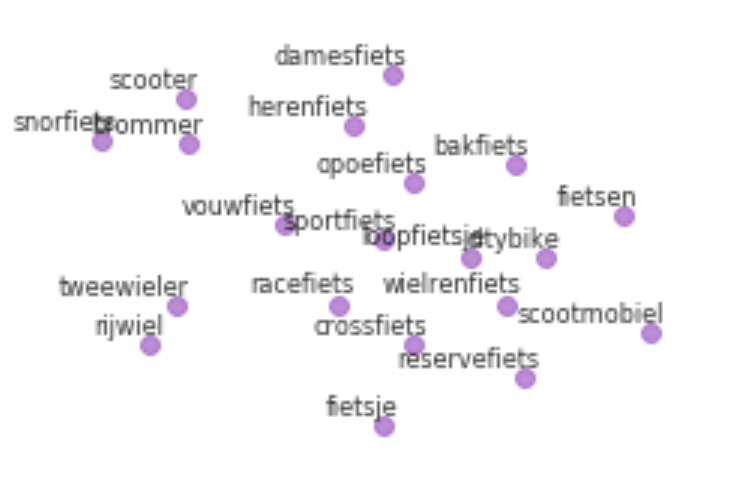
\includegraphics[width=\linewidth,height=\textheight, keepaspectratio]{fiets}}
\end{frame}

%the model has learned that fiets is similar to racefiets, wielrenfiets, rijwiel - and different from the animal department: it doesnt overlap with our kats/ dogs and birds clusters

\begin{frame}{}
	\makebox[\linewidth]{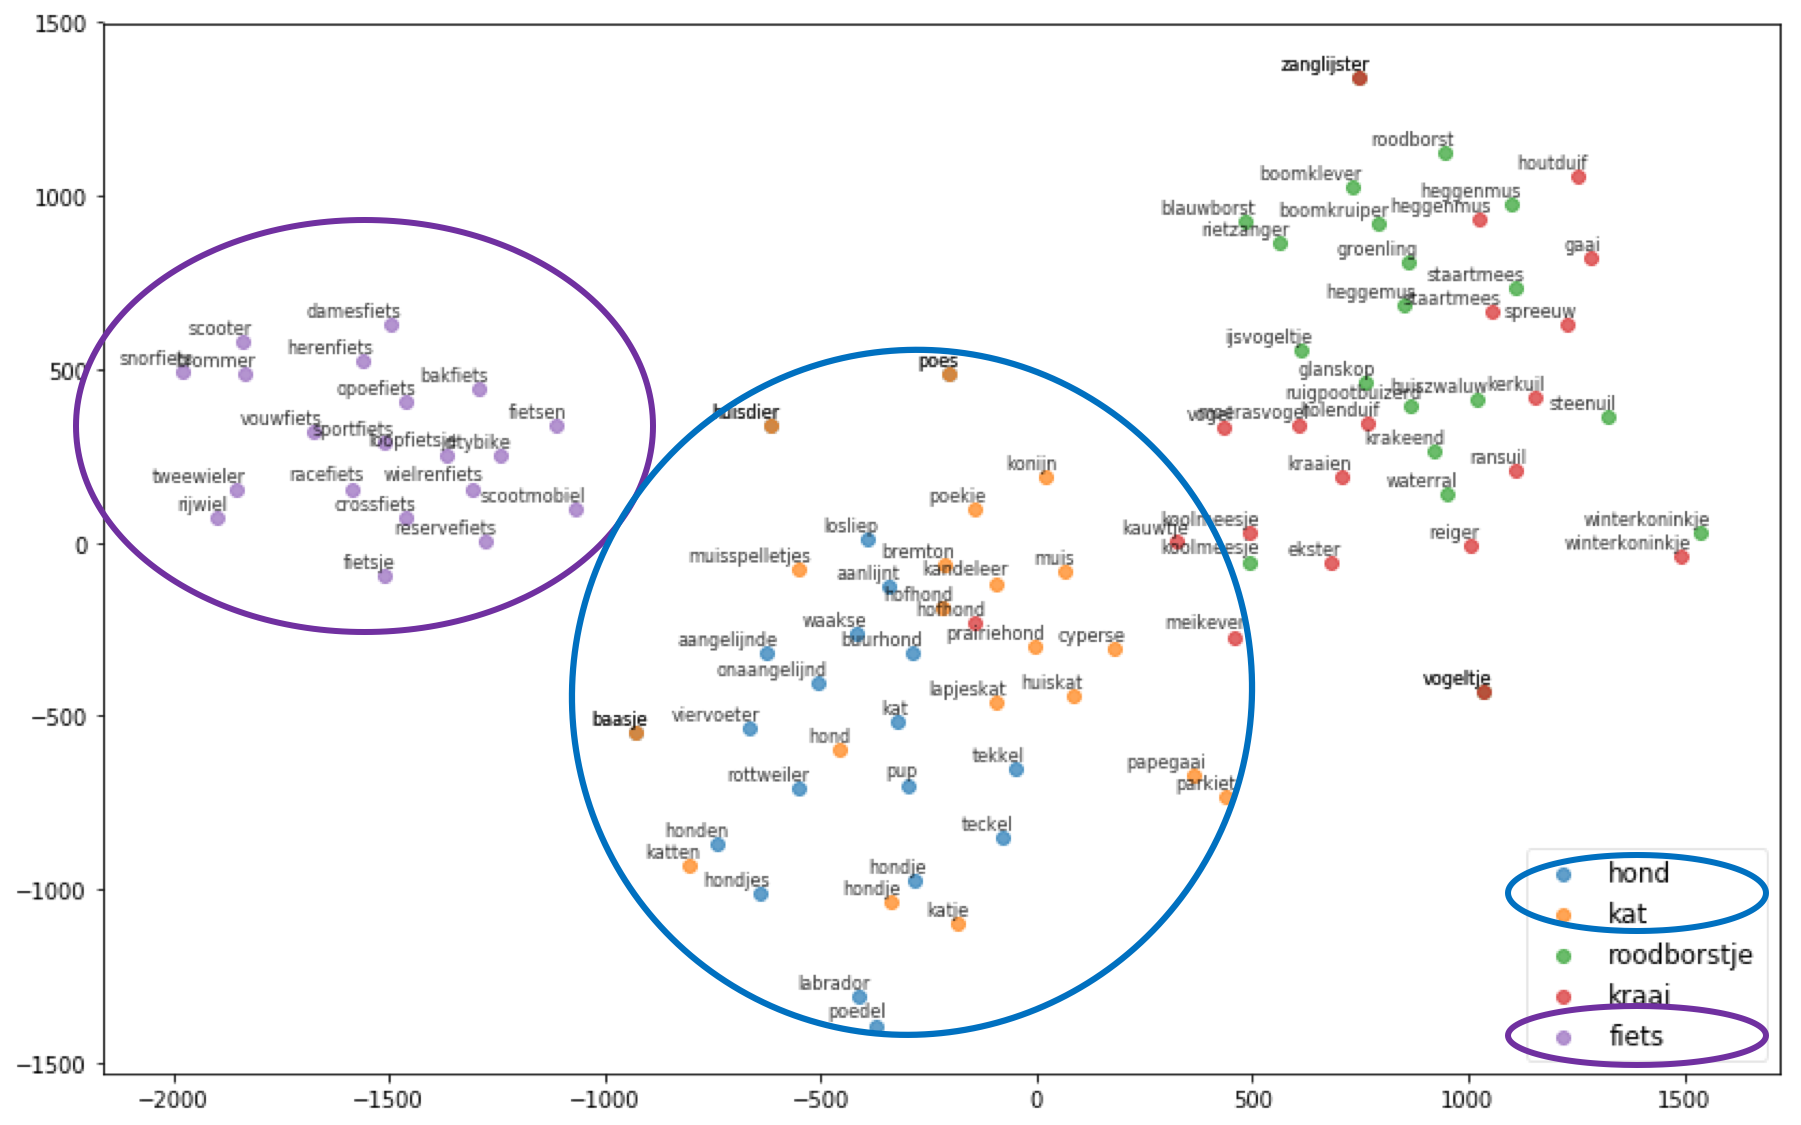
\includegraphics[width=\linewidth,height=\textheight, keepaspectratio]{visual1.png}}
\end{frame}

%the model recognizes that fiets is something else from honden and katten. Both mammals and pets, dogs and cats are quite similar and appear in the same cluster.  

\begin{frame}{}
	\makebox[\linewidth]{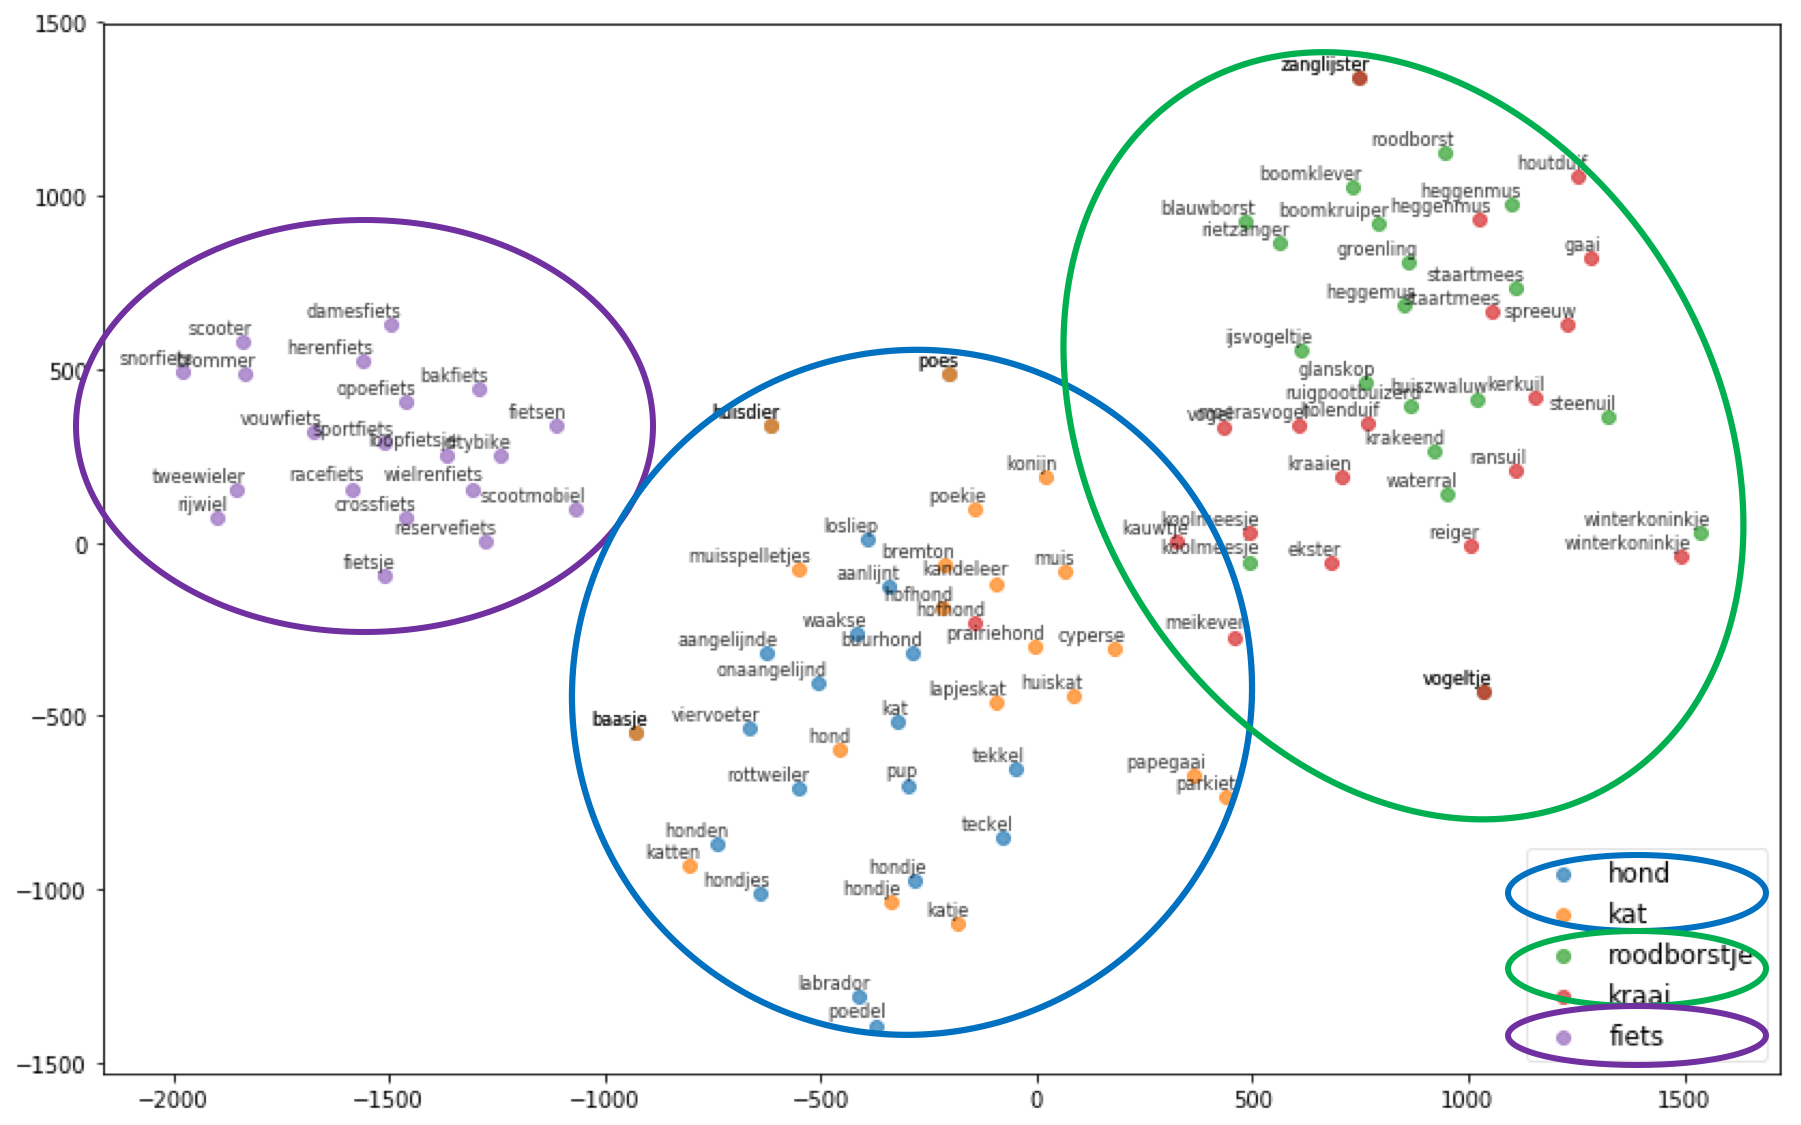
\includegraphics[width=\linewidth,height=\textheight, keepaspectratio]{visual.png}}
\end{frame}

%Finally, the model recognizes that dogs and kats are different from redbreasts and crows, with both appear in a 'bird-related' cluster.

%\begin{frame}{}
%	\makebox[\linewidth]{\includegraphics[width=\linew%idth,height=\textheight, %keepaspectratio]{bias.png}}
%\end{frame}

%Now we know that the model understands Dutch pretty well. We can now apply to model to diverse tasks that are of greater interest to communication scholars. For example, we can see whether or not our training data contains bias.When we plot the most similar words to ‘criminals, Belgians and Moroccans,  we see that Moroccans are much closer to criminals, that Belgians. THis could potentiall reveal bias in the training data.

%\subsection{Re-usability}
\begin{frame}{Re-usability}
	Re-usability of the Amsterdam Embedding Model
\end{frame}

%\subsection{Availability of model and code}
\begin{frame}{Re-usability}
	\begin{block}{Reusing model and data}
		\begin{enumerate}
			\item See \url{https://github.com/annekroon/amsterdam-embedding-model}
			\item Open access to all the code
		\end{enumerate}
	\end{block}
\end{frame}


\begin{frame}[standout]
	Disclaimer: I cannot give a full overview of the whole topic of deep learning here -- that's a whole (extensive) course in itself. But embeddings are closely related, that's why we at least will at least get out feet wet a bit.
\end{frame}


\setbeamercovered{transparent}

\begin{frame}[plain]
	\printbibliography
\end{frame}



\end{document}
